%+++++++++++++++++++++++++++++++++++++++++++++++++++++++++++++++
% SUMMARY    : Perceptrons Continued, Introduction to SVM, XPLs 
%            : University of Southern Maine 
%            : @james.quinlan
%            : Cody Savage - Lecture 7
%+++++++++++++++++++++++++++++++++++++++++++++++++++++++++++++++
\section*{Objectives}
\begin{outline}
    \1 Perceptrons Continued
    \1 Introduction to SVM
    \1 XPLs
\end{outline}

\rule[0.0051in]{\textwidth}{0.00025in}
% ----------------------------------------------------------------

\section{Perceptrons Continued}
The Perceptron\cite{rosenblatt1958perceptron} is part of a family of machine learning algorithms known as \textit{supervised learning} algorithms.

\subsection{Supervised vs Unsupervised Learning Algorithms}
A \textit{supervised learning} algorithm takes in labeled data, from which relationships between the desired output corresponding to the desired inputs are already known, from which the algorithm can make predictions on new, unlabeled data.

Meanwhile, an \textit{unsupervised learning} algorithm takes in unlabeled data, from which it is expected to find relationships and patterns among the data. For our current purposes, let's focus on the different categories of \textit{supervised learning} algorithms.

\subsection{Types of Supervised Learning Algorithms}
The two primary types of supervised learning algorithms are \textit{regression} algorithms and \textit {classification} algorithms.

\subsubsection{Regression Algorithms}
Regression algorithms, given an input $x$, maps it to a $y$, such that
\[
    y \in \mathbb{R}.
\]
That is, $x$ is mapped to a real number.

\subsubsection{Classification Algorithms}
Classification algorithms, given an input $x$, maps it to a $y$, such that
\[
    y \in \{C_1, C_2, \dots, C_n\}.
\]
That is, $x$ is mapped to $C_i$, out of $n$ possible categories.
Coincidentally, the Perceptron algorithm belongs to this category. More specifically, it is a \textit{binary classification} algorithm, where 
\[
    y \in \{-1, 1\}.
\]

\subsection{Perceptrons and Linear Separability}
The Perceptron algorithm assumes that the data it takes in is \textit{linearly separable}.

A set of data $D$, such that
$
    D = \{(x_1,y_1), \dots,(x_n, y_n)\},
$, $
    x_i \in \mathbb{R}^p,
$, and $
    y \in \{-1, 1\}.
$ is \textit{linearly separable} if and only if one can draw a hyperplane between the two sets, such that
\[
    y_i(w^\perp x +b) > 0,
\] \[
    \forall x_i, y_i.
\]
Recall that the sign of $w^\perp x+b$ tells us whether vector $x$ is `above', `below', or `on' the hyperplane. Assuming the hyperplane obtained via the Perceptron is a solution, then the sign should match the sign of the category, so if we were to multiply the category with the equation, we'll either be multiplying two positive or negative numbers together, and we should therefore always obtain a positive number.

\subsection{The Set of all Decision Functions}
Assuming that the set given to it is linearly separable, the Perceptron algorithm is guaranteed to obtain \textit{a solution}, a hyperplane that successfully splits the two classes. However, as we can see here, this solution is not guaranteed to be the \textit{optimal solution}. Consider the following dataset and decision boundary:

\begin{tikzpicture}
	\begin{axis}[
		xlabel=$x$,
		ylabel=$y$,
        xmin=-1,
        xmax=1,
        ymin=-1,
        ymax=1
	]
	\addplot [color=blue, only marks, mark=+] coordinates { 
    (-0.5, 0.5)
    (-0.2, 0.25)
    (0.75, 0.5)
    };
    \addplot [color=red, only marks, mark=-] coordinates { 
    (0.5, -0.5)
    (0, -0.6)
    (0.25, -0.75)
    };
    \addplot[no marks] coordinates {
		(-0.5, -1)
		(1, 0.6)
	};
	\end{axis}
\end{tikzpicture}

As it can be seen, while the feature vectors in the dataset are correctly categorized, the way the plane lies leaves very little room for error, and appears prone to misclassifications.

\begin{tikzpicture}
	\begin{axis}[
		xlabel=$x$,
		ylabel=$y$,
        xmin=-1,
        xmax=1,
        ymin=-1,
        ymax=1
	]
	\addplot [color=blue, only marks, mark=+] coordinates { 
    (-0.5, 0.5)
    (-0.2, 0.25)
    (0.75, 0.5)
    };
    \addplot [color=red, only marks, mark=-] coordinates { 
    (0.5, -0.5)
    (0, -0.6)
    (0.25, -0.75)
    };
    \addplot[no marks] coordinates {
		(-1, -0.5)
		(1, 0)
	};
	\end{axis}
\end{tikzpicture}

Meanwhile, this hyperplane splits the two halves of the feature space way more evenly, leaving more of a margin between the closest feature vectors to the plane. There is an infinite number of possible solutions, an infinite number of possible hyperplanes, and therefore an infinite number of possible \textit{decision functions}, which take the form
\[
    h(x) = sign(w^\perp x+b).
\]
If the hyperplane is the set of all points such that $w^\perp x+b=0$, or, the set of all points in the hyperplane, then the sign of $w^\perp x+b$ when non-zero tells us whether or not we are 'above' or 'below' the plane, and as a result, which category we belong to. From this, we can define the set of all possible decision functions,
\[
    H = \{h_1, h_2, \dots, h_n\}.
\]

\subsection{Limitations of perceptron}
\begin{itemize}
    \item Fails on non-linearly separable data.
    \item Single-layer only.
\end{itemize}

\section{Introduction to SVM}
As the previous section shows, an 'optimal' hyperplane maximizes the margin between the closest feature vector and the plane. To better maximize this margin, we'll introduce a new machine learning algorithm called the \textit{Support Vector Machine}\cite{scholkopf2002learning}\cite{vapnik1998statistical}, or \textit{SVM} for short.

The SVM is what is known as a \textit{maximum margin classifier}, which means that it is \textit{guaranteed} to find the maximum margin separating hyperplane, which is what we have decided to define as the most 'optimal' hyperplane for our purposes.

\subsection{SVM Prerequisites}
Before we delve into the specifics of the SVM algorithm, we must define an important linear algebra operation: \textit{projection}.

In the most literal sense, 'projecting' one vector onto another gives us the magnitude of the first vector in the direction of another, as if you sat the first above the second in the same plane and shined a light over it- the projection is its 'shadow' (like the example below).

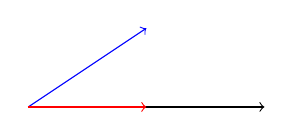
\begin{tikzpicture}
	\draw[->] (0, 0) -- (3, 0);
    \draw[blue, ->] (0, 0) -- (1.5, 1);
    \draw[red, ->] (0, 0) -- (1.5, 0);
\end{tikzpicture}

Let $u$ and $v$ be two vectors of some kind, and let us project the first onto the second. If a vector can be defined as a unit direction vector multiplied by some magnitude, we can take the direction of the resulting projection to be the unit vector of the vector we're projecting onto, $\hat{v}$ in this case.

To obtain the magnitude, let us examine the definition of the dot product.
\[
    u \cdot v = |u||v|cos\theta
\]
The dot product can be defined as the magnitudes of both vectors, multiplied by the cosine of the angle between them. Dividing both sides by $|v|$, we obtain
\[
    \frac{u \cdot v}{|v|} = |u|cos\theta.
\]
As it so happens, $|u|cos\theta$ represents the magnitude of $u$ in the direction of $v$. For example, if $u$ and $v$ are parallel, the angle between them is zero, the cosine of zero is 1, and we get the full magnitude of $u$. If $u$ and $v$ are perpendicular, the angle between them is $\frac{\pi}{2}$, and the cosine of that is zero, so there is no magnitude of $u$ in the direction of $v$.

Putting both together, we can define projection to be
\[
    proj_vu = (\frac{u \cdot v}{|v|})\hat{v} = (\frac{u \cdot v}{|v|})\frac{v}{|v|}.
\]

From this, we can also obtain the component of $u$ \textit{perpendicular} to $v$, $u^\perp$, by subtracting the projection from $u$,
\[
    u^\perp = u - proj_vu.
\]
% ----------------------------------------------------------------

\section{XPL's}
1.) Modify the perception code to add a counter to see how many updates it takes to obtain any solution.











\begin{figure}
    \centering
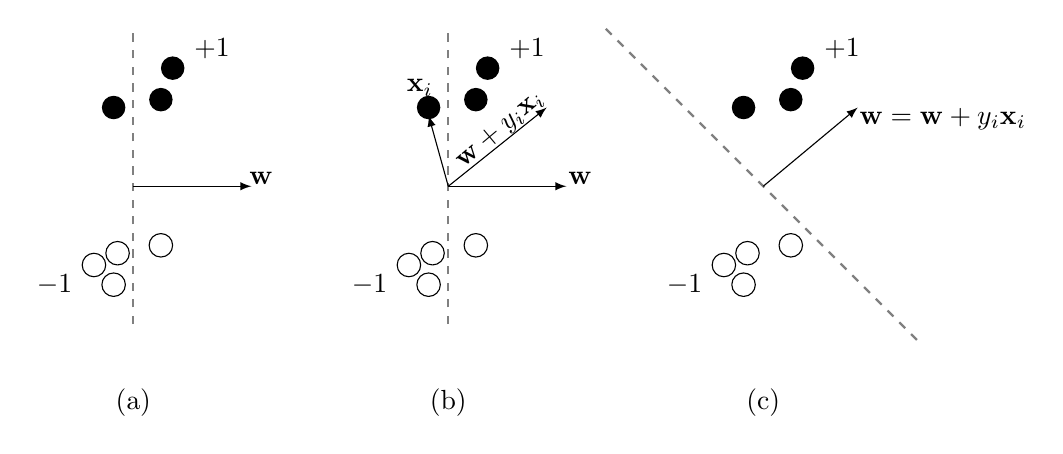
\begin{tikzpicture}

% Leftmost figure
\draw[thick, gray, dashed] (0, -1.75) -- (0, 2);
\node at (0, -2.75) {(a)};

\node at (0.5, 1.5) [circle, fill, inner sep=3.0pt] {};
\node at (0.35, 1.1) [circle, fill, inner sep=3pt] {};
\node at (-0.25, 1.0) [circle, fill, inner sep=3pt] {};

\node at (-0.25, -1.25) [ circle, draw, inner sep=3pt] {};
\node at (-0.5, -1) [circle, draw, inner sep=3pt] {};
\node at (-0.20, -0.85) [circle, draw, inner sep=3pt] {};
\node at (0.35, -0.75) [ circle, draw, inner sep=3pt] {};

 \node at (1, 1.5) [above] {$+1$};
 \node at (-1, -1.0) [below] {$-1$};
\node at (1.350, 0.1) [right] {${\bf w}$};
\draw[-latex] (0.0, 0.0) -- (1.5, 0.0);




% Middle figure
\draw[thick, gray, dashed] (4, -1.75) -- (4, 2);
\node at (4, -2.75) {(b)};
\node at (0.5+4, 1.5) [circle, fill, inner sep=3.0pt] {};
\node at (0.35+4, 1.1) [circle, fill, inner sep=3.0pt] {};
\node at (-0.25+4, 1.0) [circle, fill, inner sep=3.0pt] {};

\node at (-0.25+4, -1.25) [ circle, draw, inner sep=3pt] {};
\node at (-0.5+4, -1) [ circle, draw, inner sep=3pt] {};
\node at (-0.20+4, -0.85) [circle, draw, inner sep=3pt] {};
\node at (0.35+4, -0.75) [ circle, draw, inner sep=3pt] {};

\node at (5, 1.5) [above] {$+1$};
\node at (3, -1.0) [below] {$-1$};


% Vector W
\node at (5.4, 0.1) [right] {${\bf w}$};
\draw[-latex] (4, 0) -- (5.5, 0);

% vector x
%\draw[-latex] (4, 0) -- (4.5, -0.65);
%\node at (4.3, 0.3) [above] {$x$};

% \node at (4, 1) [above] {$x$};
% \draw[-latex, dashed] (5, 0) -- (4.75, -0.88);
\node at (3.35, 1.25) [right] {${\bf x}_i$}; % {\bf w}_k - {\bf x}
\draw[-latex] (4, 0) -- (3.75, 0.90);
\node at (4.05, 0.2) [right, rotate=40] {${\bf w} + y_i{\bf x}_i$};

% \draw[-latex] (5.5, 0) -- (5.25, 1.0);
% \draw[-latex, dotted] (4, 0) -- (5.25, 1.0);

\draw[-latex] (4, 0) -- (5.25, 1.0);

 


% Rightmost figure
\draw[thick, gray, dashed] (6, 2) -- (10, -2);
\node at (8, -2.75) {(c)};
\node at (0.5+8, 1.5) [circle, fill, inner sep=3.0pt] {};
\node at (0.35+8, 1.1) [circle, fill, inner sep=3.0pt] {};
\node at (-0.25+8, 1.0) [circle, fill, inner sep=3.0pt] {};

% hollow circles
\node at (-0.25+8, -1.25) [ circle, draw, inner sep=3pt] {};
\node at (-0.5+8, -1) [ circle, draw, inner sep=3pt] {};
\node at (-0.20+8, -0.85) [circle, draw, inner sep=3pt] {};
\node at (0.35+8, -0.75) [ circle, draw, inner sep=3pt] {};

\draw[-latex] (0+8, 0) -- (0 + 9.2, 1.0);
\node at (9, 1.5) [above] {$+1$};
\node at (7, -1.0) [below] {$-1$};
%\node at (-1.0, 1.10) [above] {+1};
%\node at (1, -1.0) [below] {-1};
% \draw[-latex] (4, 0) -- (5.25, 1.0);
\node at (9.1, 0.85) [right] {${\bf w} = {\bf w} + y_i{\bf x}_i$};
%\node at (9.1, 0.85) [right] {${\bf w}_{k+1}$};

\end{tikzpicture}
   
    \caption{Illustration of a one step update using Algorithm \ref{alg:perceptron}.  (a) The hyperplane defined by ${\bf w}$ misclassifies one hollow circle and one filled circle. (b) Hyperplane is updated since ${\bf x}_i$ was misclassified. (c) Updated hyperplane, ${\bf w} + y_i{\bf x}_i$, that separates the two classes.}
    \label{fig:perceptron}
\end{figure}

\pagebreak
\bibliographystyle{plain}
\bibliography{references}
